\section{Introduction to Graphs and Learning on Graphs}\label{sec:intro-graph}
\subsection{Basic definitions}
%\marginnote{Hi}
%\begin{marginfigure}
%	\includegraphics[width=\textwidth]{manwoman.jpg}
%\end{marginfigure}

\begin{definition}[Graph] \label{def:graph}
A graph $G = (V, E)$ is defined by a set of nodes $V$ and a set of edges between these nodes. We denote an edge going from $u \in V$ to $v \in V$ as $(u, v) \in E$.
\end{definition}
\begin{marginfigure}
	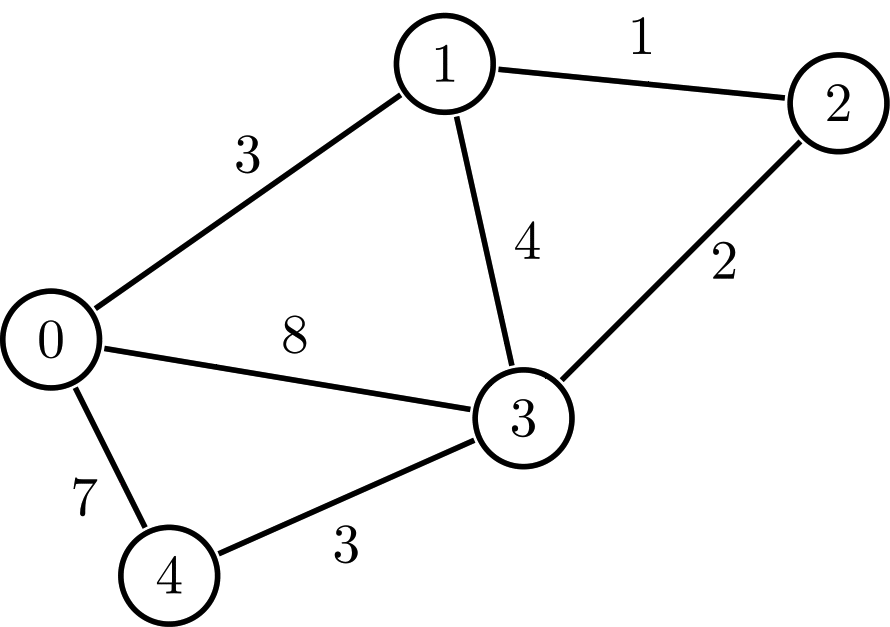
\includegraphics[width=\textwidth]{undirected-graph.png}
	\caption{Undirected graph with ordered edges and nodes}
	\label{fig:undirected-graph}
\end{marginfigure}
Note that definition \ref{def:graph} is general, and most of the times we are only concerned with \textit{simple graphs}, which have the following properties:
\begin{itemize}
	\item[$\diamond$] For any two nodes in the set $V$, there exists at most one edge between them.
	\item[$\diamond$] There are no self-loops, i.e for any $u \in V$, $(u, u) \notin E$.
	\item[$\diamond$] All edges of the graph are \textit{undirected}, i.e for $u, v \in V$, $(u, v) \in E \Leftrightarrow (v, u) \in E$.
\end{itemize}
\begin{definition}[Adjacency Matrix] \label{def:adjacency}
For a simple graph $G = (V, E)$, the adjacency matrix $\mathbf{A} \in \mathbb{R}^{|V| \times |V|}$ is a square matrix with $A_{uv} = 1$ if there is an edge from vertex $u$ to $v$, and $A_{uv} = 0$ otherwise.
\end{definition}
\marginnote{
\[\mathbf{A} = \begin{bmatrix}
	0 & 1 & 0 & 1 & 1 \\
	1 & 0 & 1 & 1 & 0 \\
	0 & 1 & 0 & 1 & 0 \\
	1 & 1 & 1 & 0 & 1 \\
	1 & 0 & 0 & 1 & 0
\end{bmatrix} \]
\begin{center}
The adjacency matrix for Fig \ref{fig:undirected-graph}.
\end{center}
}
Since we are dealing with simple graphs, some immediate consequences are that
\begin{itemize}
	\item[$\diamond$] $\mathbf{A}$ is symmetric, i.e $\mathbf{A}^T = \mathbf{A}$.
	\item[$\diamond$] $A_{uu} = 0 \; \forall \; u \in V$, i.e all diagonal elements are zero.
\end{itemize}
Notice that since we are defining the graph in terms of the matrix $\mathbf{A}$, we need to order the nodes prior to the representation (See Fig \ref{fig:undirected-graph}). An extension to definition \ref{def:adjacency} occurs when we allow the use of weighted edges, and in that case for $u, v \in V$, ${A}_{uv} \in [0, 1]$.

\subsection{Multi-relational Graphs}
We have noted three types of edges till now: undirected, directed and weighted. But for graphs, it is possible to have different types of edges. In such cases, we extend the notation to include relation type $\tau \in \mathcal{R}$ and write that $(u, \tau, v) \in E$ along with defining an adjacency matrix $\mathbf{A}_\tau$ for each type. The above class of graphs are called multi-relational, and are overall represented by an adjacency tensor $\mathcal{A} \in \mathbb{R}^{|V| \times |\mathcal{R}| \times |V|}$. Two major subsets of such graphs are:
\begin{enumerate}
	\item \textbf{Heterogeneous graphs:} We can partition the set of nodes into $k$ disjoint sets $V = \bigcup_{i=1}^k V_i$, and thus we have types imbued on nodes. 
	Usually in such graphs, we pose constraints on edges, for example they connect nodes of different types only (\textit{multipartite graphs}).
	\begin{marginfigure}
		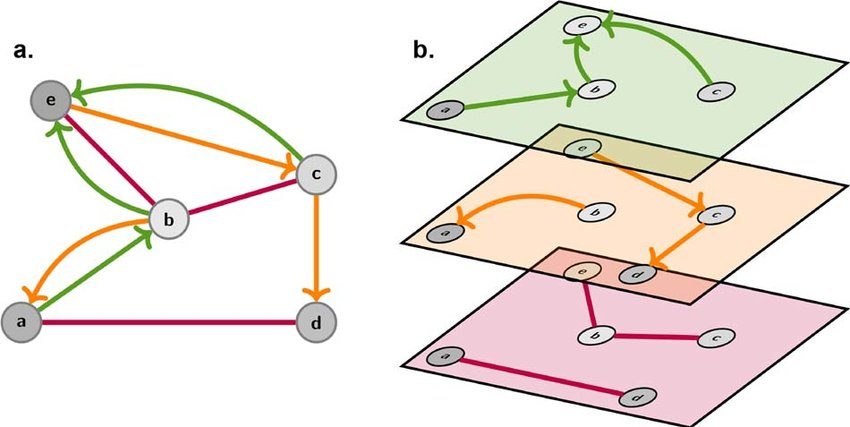
\includegraphics[width=\textwidth]{multi-relational-graph.png}
		\caption{Layered multiplex graph. Source: \cite{multiplexgraph}}
		\label{fig:multi-relational-graph}
	\end{marginfigure}
	\item \textbf{Multiplex graphs: }We can decompose such graphs into a set of layers (see Fig \ref{fig:multi-relational-graph}), and each node is in every layer with each layer possessing a unique relation. Edges will be present intra-layer and inter-layer.
\end{enumerate}

\subsection{Information representation}
Usually we have features representing graph-level features - may it be on nodes, edges or the entire graph itself. The most common one is node-level, and we associate an $m-$dimensional feature vector with each node, thus overall having a matrix $\mathbf{X} \in \mathbb{R}^{|V| \times m}$.

Now, let's go over some common graphical learning tasks.
\subsection{Node Classification}
	\begin{marginfigure}
	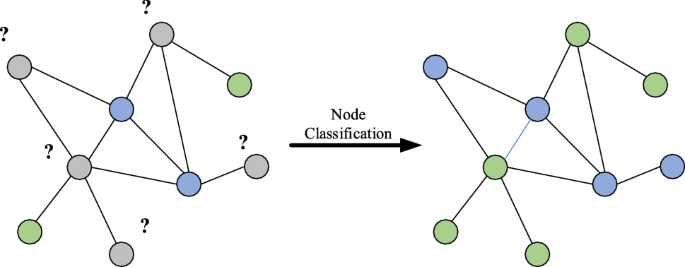
\includegraphics[width=\textwidth]{node-classification.png}
	\caption{Example of node classification. Source: \cite{node-classification-survey}}
	\label{fig:node-classification}
\end{marginfigure}
The goal of node classification is to predict a label $y_u$ associated with all nodes $u \in V$ when we have been only given the true labels of a subset of the nodes $V_{train} \subset V$. A few examples in literature of the task are:
\begin{enumerate}
	\item Interactome protein function classification: \cite{graphsage}
	\item Document classification based on citation graphs: \cite{gcn}
\end{enumerate}
Though it seems similar to supervised classification, there is a difficulty that the nodes in a graph are not \textit{i.i.d.} and thus we need to model dependencies between data points. This is exactly what node classification takes a benefit of through 
\begin{enumerate}
	\item \textbf{Homophily} \cite{homophily}: Tendency of nodes to share attributes with their neighbors
	\item \textbf{Structural Equivalence} \cite{structural-equivalence}: Idea that nodes with similar local neighborhood structures will have similar labels
	\item \textbf{Heterophily}: Presumption that nodes will be preferentially connected to differently-labeled nodes
\end{enumerate}
Note that, the only part of the network we don't access is the labels of the test nodes. We still have access to the structural information, and thus our task is \textbf{semi-supervised}.
\subsection{Link Prediction}
This task is related to the inference of edges between nodes in a graph. Given a set of nodes $V$ and an incomplete set of edges $E_{train} \subset E$, we want to infer the set $E \setminus E_{train}$. A few examples in literature of the task are:
\begin{marginfigure}
	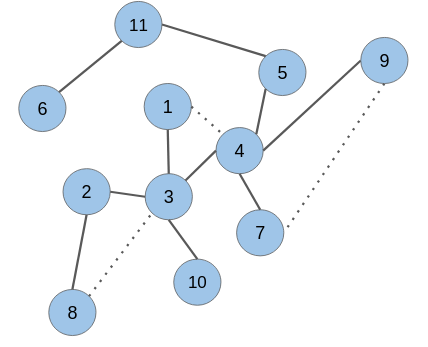
\includegraphics[width=\textwidth]{link-prediction.png}
	\caption{Example of node classification. Source: \href{https://www.analyticsvidhya.com/blog/2020/01/link-prediction-how-to-predict-your-future-connections-on-facebook/}{AnalyticsVidhya}}
	\label{fig:link-prediction}
\end{marginfigure}
\begin{enumerate}
	\item Content recommendation on social media: \cite{link-prediction-content}
	\item Modeling side-effects of drugs: \cite{link-prediction-side-effects}
\end{enumerate}
Although for simple graphs, we can have simple heuristics to give decent results \cite{link-prediction-survey-heuristic}, the task on multi-relational graphs is much more complex. \\
Much like node classification, the task boundary is smudged, and it falls under both supervised and unsupervised.
\subsection{Community Detection}
This task is the graphical analog of unsupervised learning. We want to infer latent community structures given only the input graph $G = (V, E)$. A few examples in literature of the task are:
\begin{enumerate}
	\item Uncovering functional modules in genetic interaction networks: \cite{community-detection-genetic}
	\item Fraud detection in financial transaction networks: \cite{community-detection-fraud}
\end{enumerate}
\subsection{Other popular graphical tasks}
\begin{itemize}
	\item[$\diamond$] \textbf{Graph Regression / Graph Classification}: In these tasks, we want to learn over graph data, and our dataset consists of multiple different graphs and we predict graph-wise. We can treat each graph as i.i.d and thus, the only challenge is to define useful features over graphs.
	\item[$\diamond$] \textbf{Graph Clustering} In this task, we learn an unsupervised measure of similarity between pairs of graphs.
\end{itemize}